%%%%%%%%%%%%%%%%%%%%%%%%%%%%%%%%%%%%%%%%%%%%%%%%%%%%%%%%%%%%%%%%%%%%%%
% How to use writeLaTeX: 
%
% You edit the source code here on the left, and the preview on the
% right shows you the result within a few seconds.
%
% Bookmark this page and share the URL with your co-authors. They can
% edit at the same time!
%
% You can upload figures, bibliographies, custom classes and
% styles using the files menu.
%
%%%%%%%%%%%%%%%%%%%%%%%%%%%%%%%%%%%%%%%%%%%%%%%%%%%%%%%%%%%%%%%%%%%%%%

\documentclass[12pt]{article}

\usepackage{sbc-template}

\usepackage{graphicx,url}

%\usepackage[brazil]{babel}   
\usepackage[utf8]{inputenc}

\usepackage{ulem} %para riscar potenciais deleções com o comando \sout{}
     
\sloppy

\title{Software educacional para orientação de autistas sobre comportamento no mercado de trabalho}

\author{Marcos Tadeu Magalhães Rezende\inst{1}, Pedro Oliveira Simões\inst{1}, Thiago Oliveira Gonçalves\inst{1} }


\address{Instituto de Ciencias Exatas e Informática - Pontifícia Universidade Católica de Minas Gerais  \\(PUCMINAS)
\\
  Av: Dom Jose Gaspar, 500 Coração Eucarístico – Belo Horizonte – MG – Brasil
  \email{pedro.simoes.1204205@sga.pucminas.br, mtmrezende@sga.pucminas.br}
}

\begin{document} 

\maketitle

%\begin{abstract}
%  The educational software Perceber 2, developed by Erica Borges Teixeira, contemplates pedagogical activities which may cooperate with the visual perception development of classic autist students. More specifically, it works object pairing, seriation, attribute identification and global reading. In this paper, it is proposed a new version for this project oriented to labour market activities.
%\end{abstract}

%se animar de pôr abstract, descomente acima
     
\begin{resumo}
  O software educacional Perceber 2, desenvolvido por Erica Borges Teixeira, contempla atividades pedagógicas que podem colaborar com o desenvolvimento da percepção visual de estudantes autistas clássicos. Mais especificamente, são trabalhados emparelhamento de objetos, seriação, identificação de atributos e leitura global. Neste trabalho, é proposta uma nova versão para este projeto orientada para atividades do mercado do trabalho.
\end{resumo}

\section{Introdução}

O software educacional Perceber 2, desenvolvido por Erica Borges Teixeira, contempla atividades pedagógicas que podem colaborar com o desenvolvimento da percepção visual de estudantes autistas clássicos. Na monografia da autora, foi descrito todo o processo de criação do aplicativo, incluindo o processo de software e um detalhamento sobre o transtorno de espectro autista, que foi acompanhado por professores especializados. Com isso, o produto final foi um aplicativo de tablet em Android gratuito que possui atividades para aumentar a percepção visual de estudantes autistas, trabalhando com emparelhamento de objetos, seriação, identificação de atributos e leitura global \cite{Perceber2}.

Este trabalho possui como objetivo propor uma nova versão para este projeto orientada para atividades do mercado do trabalho.

\section{O Autismo}

O autismo é classificado como um de vários Transtornos Globais de Desempenho, caracterizado pelo desenvolvimento acentuadamente prejudicado na interação social e comunicação, além de um repertório marcantemente restrito de atividades e interesses.

Estes transtornos recebem diferentes nomeclaturas conforme sua gravidade. Alguns exemplos incluem a Síndrome de Rett, Transtorno ou Síndrome de Asperger e Transtorno Desintegrativo da Infância.

Segundo \cite{leopoldino:17}, "Diagnóstico tardio, restrições de acesso à educação, negação de terapias tradicionais e alternativas e baixa renda familiar estão entre os principais fatores que influenciam negativamente a construção de conhecimento e autonomia dos autistas e, consequentemente, sua probabilidade de aceitação no mercado laboral".

Apesar de autistas serem tratados com desconfiança devido a seu comportamento social atípico, \cite{schmidt:15} reforça que as competências além da média deste perfil de público, como habilidade com dispositivos computacionais, honestidade, integridade, pontualidade, competência técnica, persistência e lealdade devem ser considerados pelos empregadores do mercado de trabalho.

Portanto, uma preparação apropriada do indíviduo diagnosticado com algum grau do Transtorno do Espectro Autista que realçe suas competências, mas simultaneamente incentive-o a compreender seus defeitos e como aprender a lidar com eles para ser uma boa pessoa e um bom profissional é fundamental para a inserção deste perfil de público no mercado de trabalho atual.

\section{Metodologia}

O software Perceber usa como referência em suas atividades ambientes e objetos de casa. Esta adaptação pretende usar como referência ambientes e objetos típicos do mercado do trabalho, como escritório, sala de reunião, sala de conferência, espaço social.

O objetivo principal é orientar o colaborador acerca de comportamento em espaços de trabalho em relação a convivência e socialização, horário de trabalho, noções de espaço ou comportamento em casa em períodos de home-office.

\subsection{Atividades}
\begin{itemize}
\item Identificação de objetos: O colaborador precisa identificar um objeto solicitado entre vários;
\item Identificação de atributos: O colaborador deve identificar um objeto entre vários semelhantes conforme o atributo solicitado;
\item Seriação: O colaborador deve organizar um grupo de objetos de acordo com o grau de relevância do contexto no qual estão inseridos;
\item Leitura Global: O colaborador deve saber identificar, entre vários nomes, o correspondente ao objeto mostrado no centro da tela;
\item Emparelhamento de objetos: O colaborador precisa organizar sua mesa de escritório com vários objetos;
\item Emparelhamento de horário: O colaborador deve ser capaz de organizar um grupo de atividades como reunião, desenvolvimento, pesquisa e horário vago em um quadro de horários;
\item Emparelhamento de horário home-office: Semelhante a atividade acima, mas num contexto de home-office. Explicar o quão manter-se organizado com os horários em home-office é tão fundamental quanto em trabalho presencial;
\item Dress coding: O colaborador deve saber diferenciar em um grupo de roupas qual melhor se aplica para cada ocasião. Explicar quando uma mesma peça de roupa puder ser usada em mais de um contexto, por exemplo, uso de roupas formais em home-office para estimular o trabalho como se fosse presencial.
\item Convivência: Propôr diálogos fictícios que estimulem o colaborador a se expressar: Cumprimentar os colegas de trabalho, opinar acerca de afirmações ouvidas, dar sugestões baseadas no contexto, saber se comportar ao se comunicar com superiores, saber lidar com imprevistos e mudanças na rotina de trabalho.
\end{itemize}

\subsection{Fluxo de telas}

% Nota: O \LaTeX \ coloca as imagens, tabelas e semelhantes onde ele bem entender porque cabe ao autor citá-los ao longo do texto. Consultando outros artigos, foi esta a conclusão ao qual eu cheguei

O fluxo de telas está especificado da seguinte forma: De um menu principal, representado na Figura \ref{fig:menu}, o usuário seleciona um dos botões que leva a tela de sua respectiva atividade.

O usuário também pode navegar entre as atividades sem precisar retornar ao menu ou retornar a este por meio dos botões no canto inferior das telas de atividades.

As telas de atividades são descritas a seguir.

% Esta sub-seção de Fluxo de telas não ficaria melhor como sub-seção da seção "Adaptação do Perceber 2", antes de "Telas de software"?

% \begin{figure}[h]
%    \centering
%    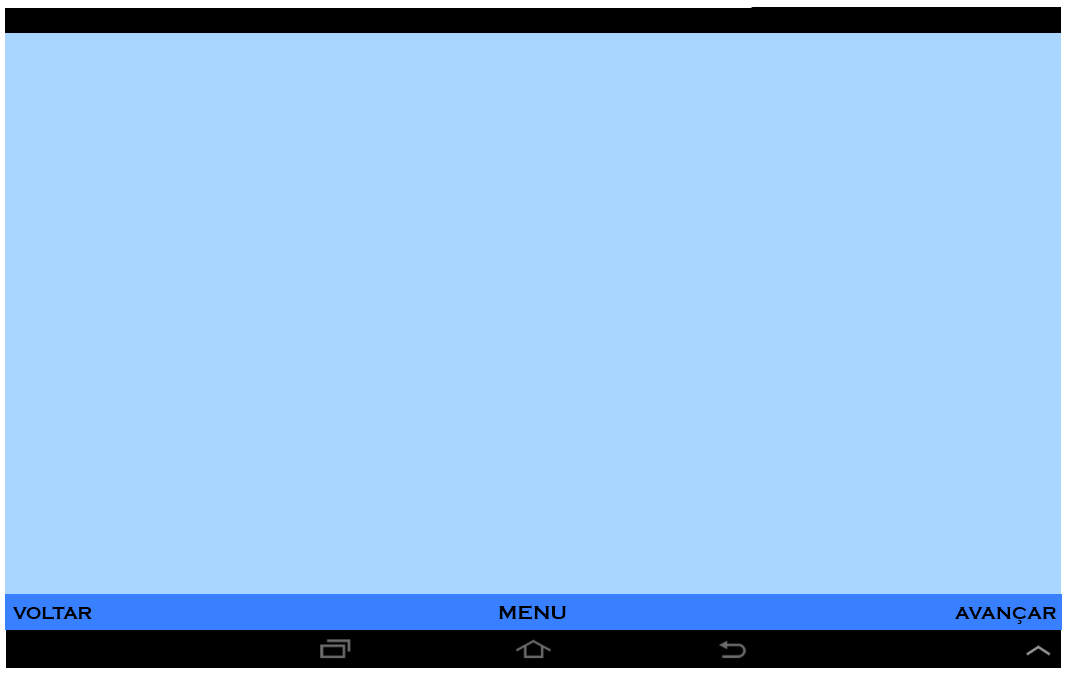
\includegraphics[width=1.0\textwidth]{template_atv1.png}
%    \caption{Template para o fundo da aplicação}
%    \label{fig:tela}
%\end{figure}

\section{Adaptação do Perceber 2}

Nesta seção estão presentes as descrições do software e das telas que se originariam da adaptação do Perceber 2. O software contempla atividades para o desenvolvimento da percepção visual de pessoas autistas em ambiente de trabalho. Mais especificamente, são trabalhadas atividades de seriação, emparelhamento de objetos, identificação de atributos e leitura global para a melhoria da percepção visual.

\subsection{Telas de Software}

As telas de software desta seção serão protótipos que mostram o visual pretendido para uma versão do software Perceber 2 adaptada para o ambiente de trabalho. O layout das telas foi mantido o mesmo, com algumas mudanças em esquema de cores e com as maiores mudanças sendo vistas na escolha dos objetos com os quais o usuário terá que interagir com.

O \textbf{Menu} principal, assim como no software original, é composto dos seguintes módulos:
\begin{itemize}
    \item Ambientação
    \item Identificação de objetos
    \item Emparelhamento de Objetos Iguais
    \item Emparelhamento de Objetos por Associação
    \item Identificação de Atributos
    \item Seriação
    \item Leitura Global
    \item Aplicabilidade Social
    \begin{itemize}
        \item Emparelhamento de horário
        \item Emparelhamento de horário home-office
        \item Dress-coding
        \item Convivência
    \end{itemize}
        
\end{itemize}
 \begin{figure}[h!]
    \centering
    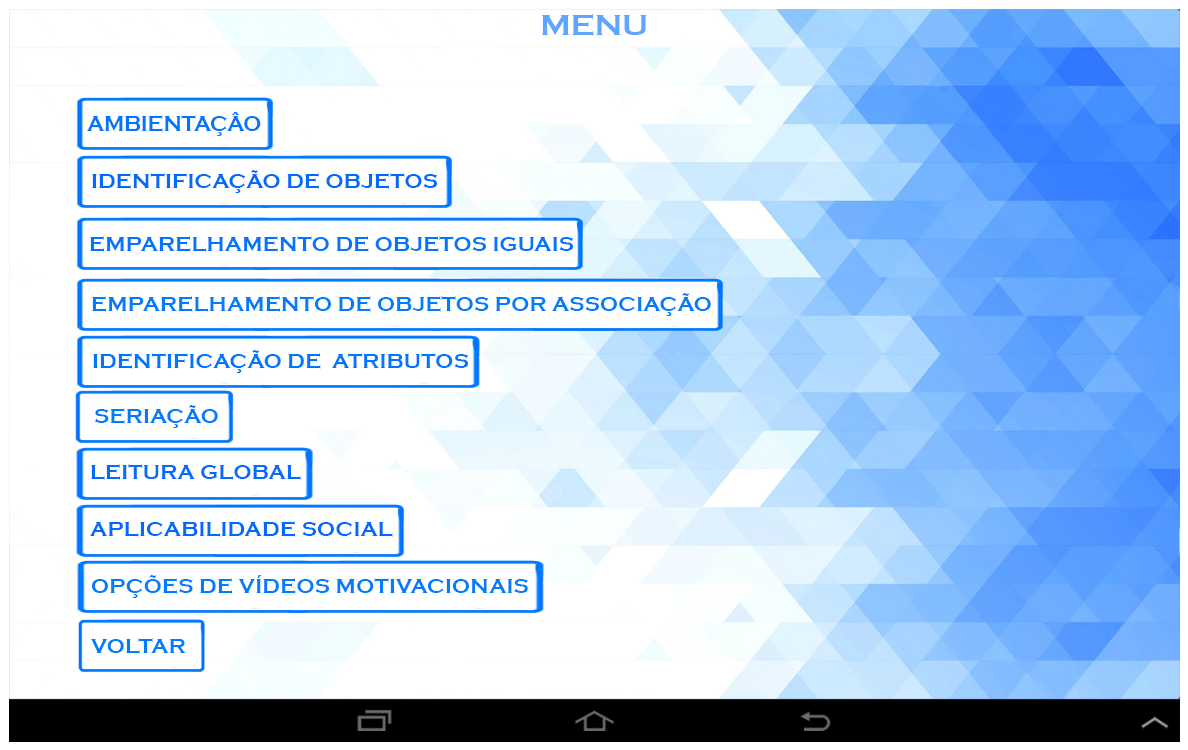
\includegraphics[width=1.0\textwidth]{menu.png}
    \caption{ Tela de menu de atividades }
    \label{fig:menu}
\end{figure}
\subsubsection{Ambientação}
O usuário começa pelas atividades de Ambientação, mostradas nas Figuras \ref{fig:ambiente_toque} e \ref{fig:ambiente_arrastar}. Esse módulo ambienta o usuário a fazer certos movimentos que ele precisará utilizar em todas as outras atividades, como arrastar e tocar. É uma atividade essencial para verificar o nível de familiaridade do usuário com as funções básicas que serão necessárias para a execução das atividades. A atividade de arrastar também possui mais de um objeto para arrastar para a lixeira, sendo recusado caso o objeto não seja designado para o local correspondente. Além disso, na figura \ref{fig:ambiente} há a atividade de escolha de ambientes, na qual o colaborador escolhe qual o ambiente próprio para a atividade em descrita.
 \begin{figure}[h!]
    \centering
    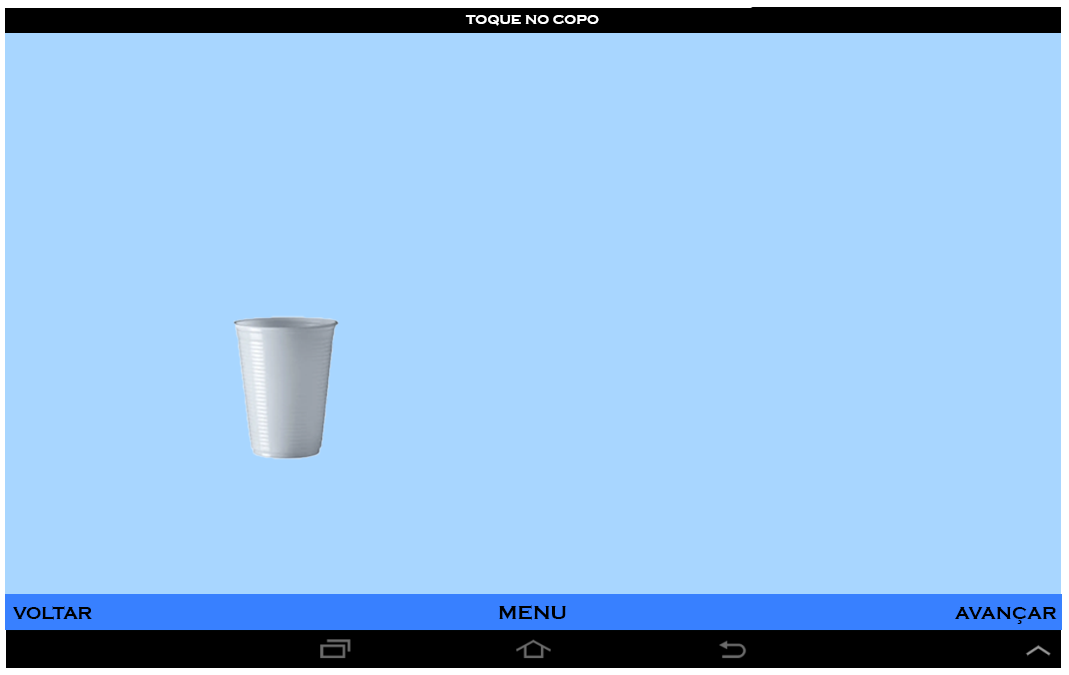
\includegraphics[width=1.0\textwidth]{ambiente_toque.png}
    \caption{Atividade de ambientação - Toque}
    \label{fig:ambiente_toque}
\end{figure}
 \begin{figure}[h!]
    \centering
    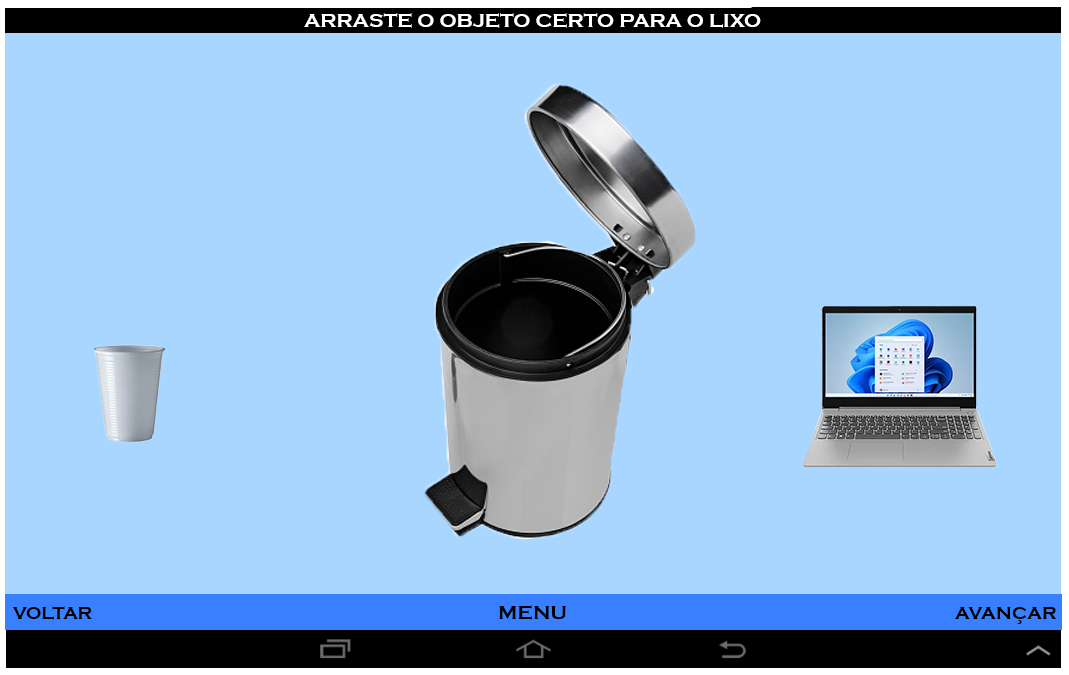
\includegraphics[width=1.0\textwidth]{ambiente_arrastar.png}
    \caption{Atividade de ambientação - Arrastar}
    \label{fig:ambiente_arrastar}
\end{figure}

 \begin{figure}[h!]
    \centering
    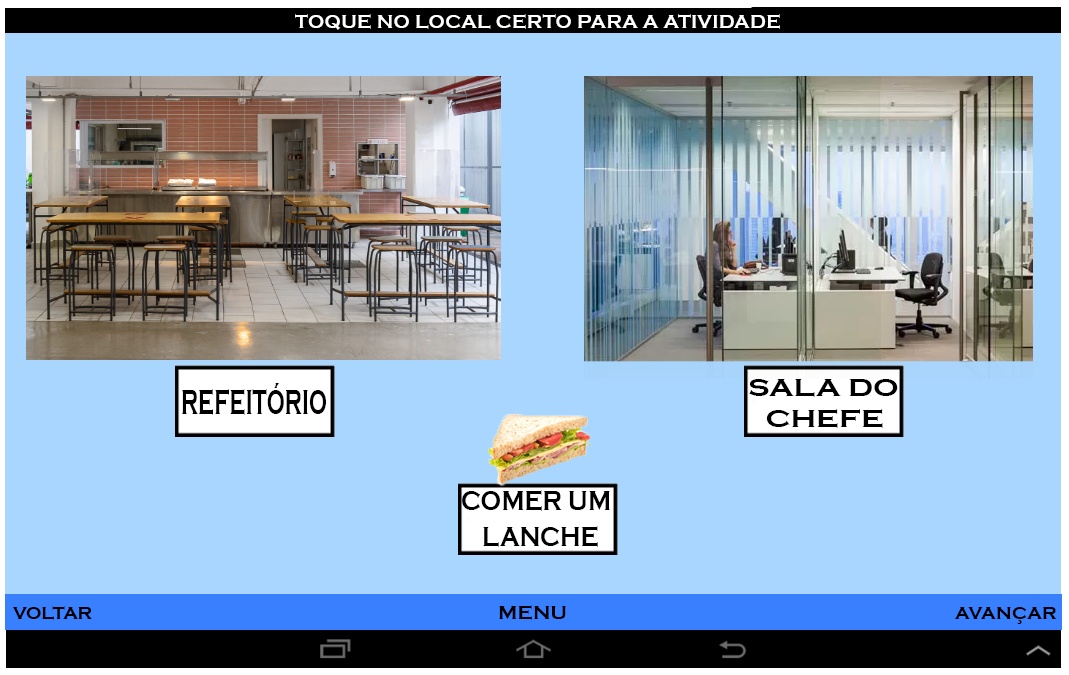
\includegraphics[width=1.0\textwidth]{ambiente.png}
    \caption{Atividade de ambientação - Ambientação}
    \label{fig:ambiente}
\end{figure}
\subsubsection{Identificação de objetos}

 \begin{figure}[h!]
    \centering
    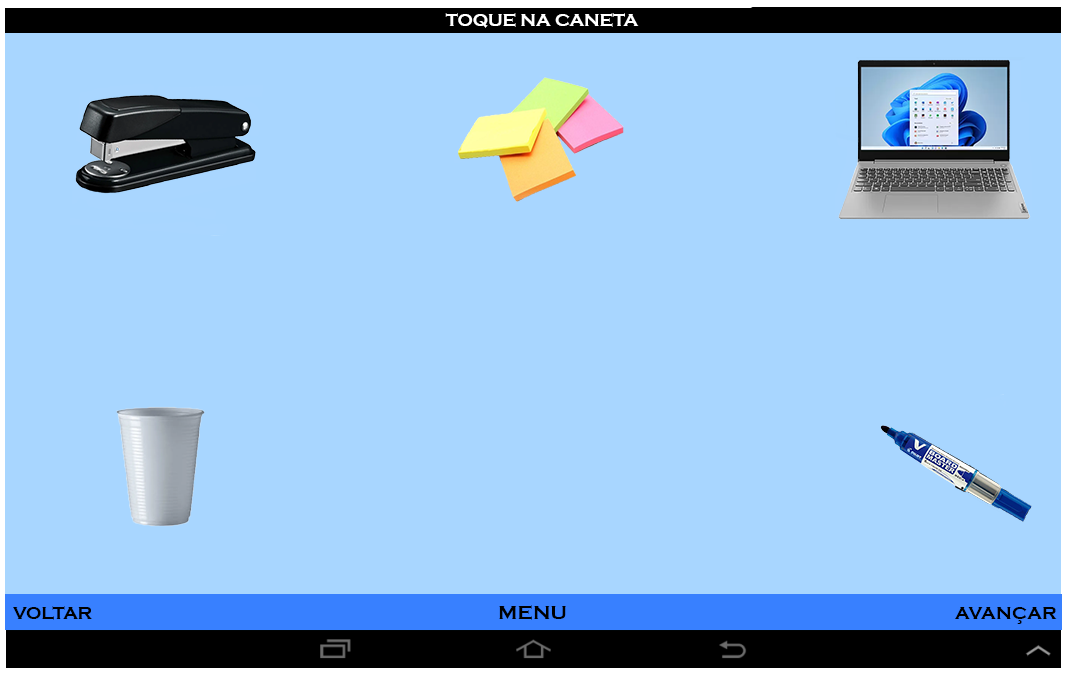
\includegraphics[width=1.0\textwidth]{identificacao_objetos.png}
    \caption{ Atividade de Identificação de Objetos}
    \label{fig:identificacao_objetos}
\end{figure}
Nesta lição o colaborador tem que tocar em um determinado objeto dentre outros, conforme apresentada na Figura \ref{fig:identificacao_objetos}. Há cinco níveis e a quantidade de objetos aumenta de
acordo com cada nível. Ao tocar no botão avançar, os objetos continuam os mesmos,
porém eles trocam de lugar, para evitar que o usuário memorize a resposta em função
da disposição dos elementos.
\subsubsection{Emparelhamento de Objetos Iguais}

 \begin{figure}[h!]
    \centering
    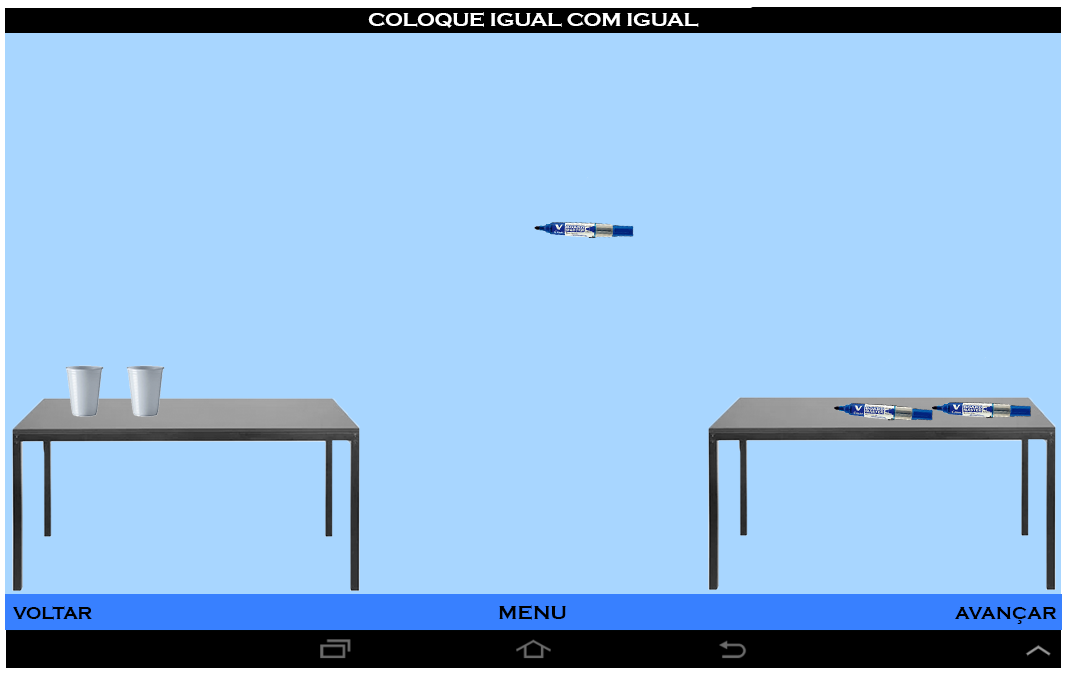
\includegraphics[width=1.0\textwidth]{emparelhamento_obj_igual.png}
    \caption{Atividade de Emparelhamento de Objetos Iguais}
    \label{fig:emparObjIgual}
\end{figure}
Na Figura \ref{fig:emparObjIgual} é mostrado um exemplo de uma atividade de emparelhamento de objetos
iguais. Essa atividade serve para que o colaborador consiga identificar objetos e colocá-los
junto aos iguais. Essa atividade possui cinco níveis. A cada toque no botão avançar, os
objetos são trocados.

\subsubsection{Emparelhamento de Objetos por Associação}

 \begin{figure}[h!]
    \centering
    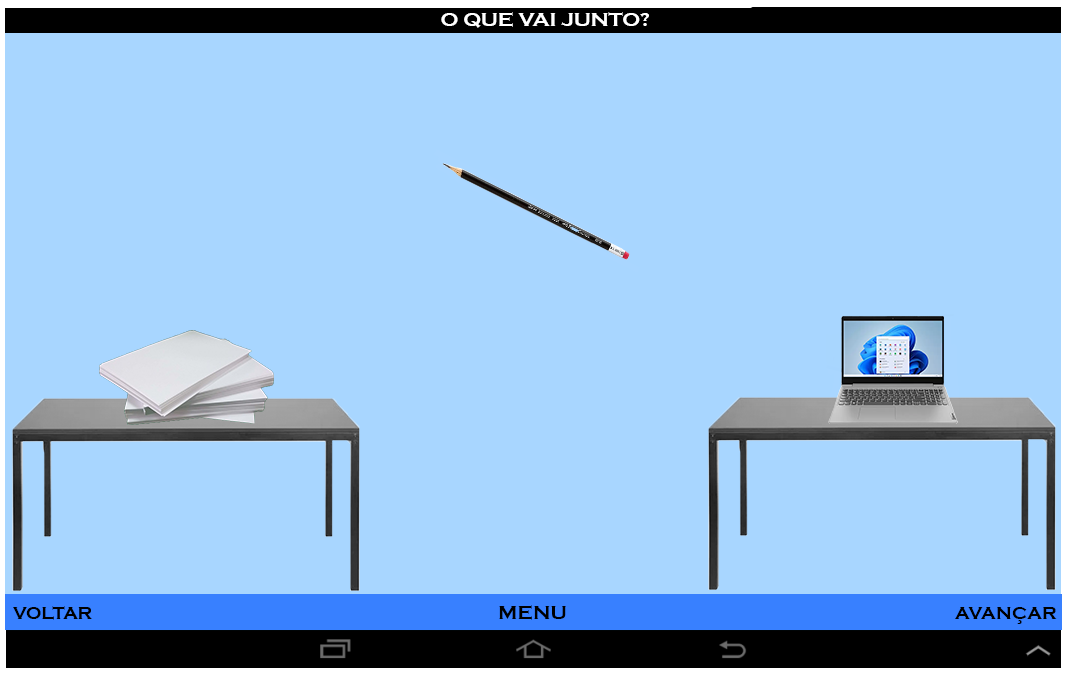
\includegraphics[width=1.0\textwidth]{emparelhamento_obj_assoc.png}
    \caption{Atividade de Emparelhamento de Objetos por Associação}
    \label{fig:emparObjAssoc}
\end{figure}
Na Figura \ref{fig:emparObjAssoc} é mostrado a atividade de emparelhamento de objetos por associação. Essa atividade funciona de maneira a fazer o colaborador arrastar o objeto que está posicionado no centro até outro objeto do mesmo contexto/funcionalidade. Essa atividade possui três níveis. A cada toque no botão avançar, os objetos são trocados.

\subsubsection{Identificação de Atributos}

 \begin{figure}[h!]
    \centering
    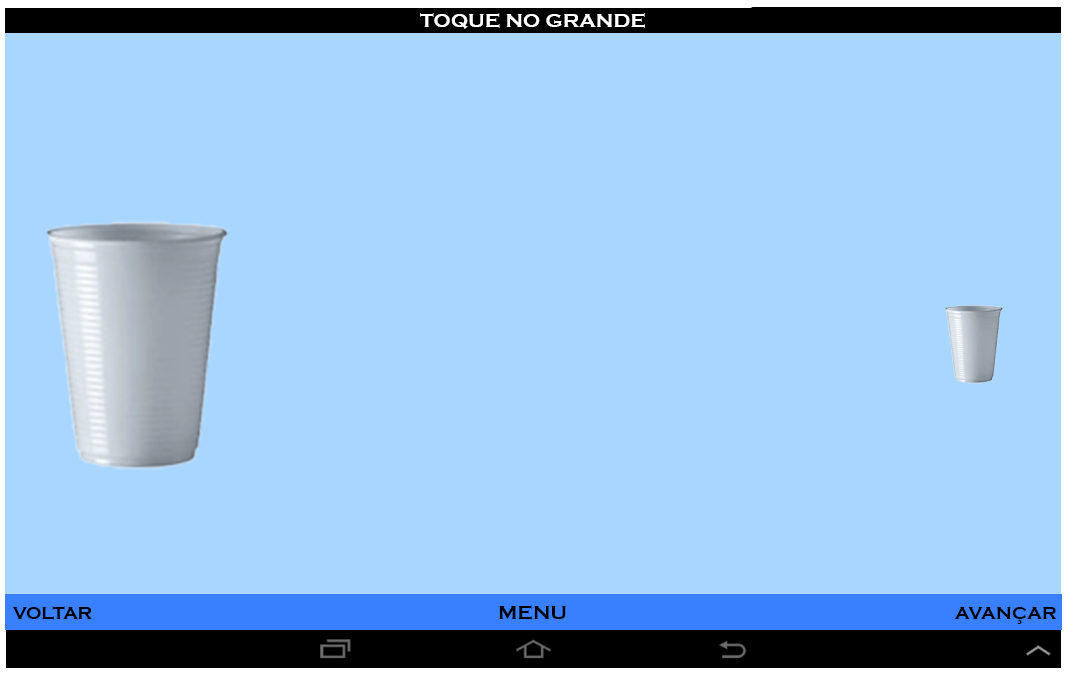
\includegraphics[width=1.0\textwidth]{identificacao_atr.png}
    \caption{ Atividade de Identicação de Atributos }
    \label{fig:identificacaoAtr}
\end{figure}

Na Figura \ref{fig:identificacaoAtr} é mostrado um exemplo de uma atividade de Identicação de Atributos. Essa atividade serve para que o colaborador entenda a diferença entre objetos iguais, mas de tamanhos diferentes. Essa atividade tem três níveis, o nível 1 aborda o atributo pequeno, o nível 2 aborda o atributo grande e o nível 3 mistura os dois. A cada toque no botão avançar, os objetos são trocados.

\subsubsection{Seriação}

 \begin{figure}[h!]
    \centering
    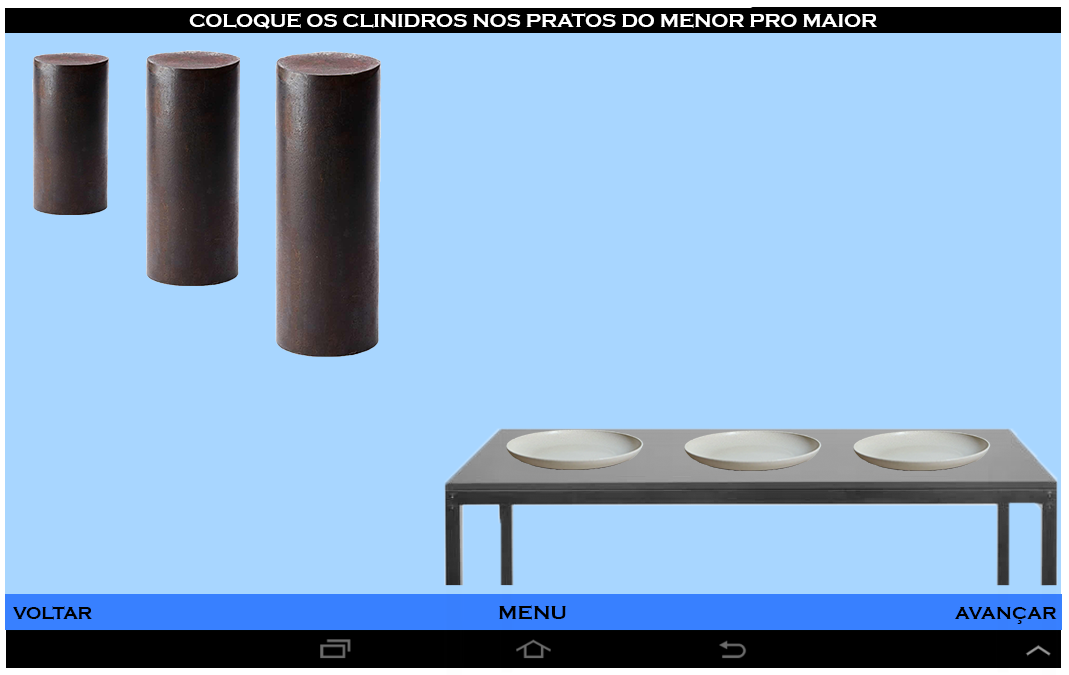
\includegraphics[width=1.0\textwidth]{seriacao.png}
    \caption{ Atividade de Seriação }
    \label{fig:seriacao}
\end{figure}

Na Figura \ref{fig:seriacao} é mostrado um exemplo de uma atividade de seriação. A proposta é que
o colaborador saiba colocar os objetos de tamanhos diferentes em ordem crescente. Essa
atividade possui cinco níveis.


\subsubsection{Leitura Global}

 \begin{figure}[h!]
    \centering
    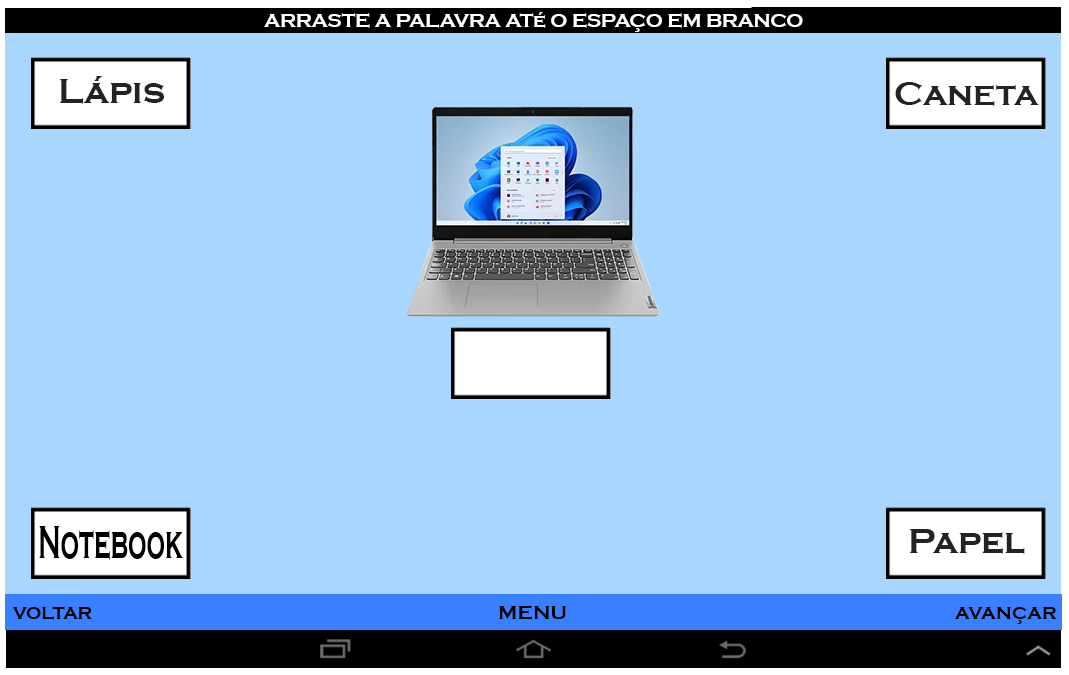
\includegraphics[width=1.0\textwidth]{leitura_global.png}
    \caption{ Atividade de Leitura Global }
    \label{fig:leitura}
\end{figure}

Na figura \ref{fig:leitura} é mostrado um exemplo de uma atividade de leitura global. Esta atividade procura ajudar o colaborador associar as palavras que foram arrastadas com as imagens que aparecem em cima da caixa de texto, a fim de permitir o colaborador apreender através de associação entre texto e imagem.

\subsubsection{Aplicabilidade Social}
O módulo de aplicabilidade social foi desenvolvido tendo em mente contextos reais em que o colaborador frequentemente se encontraria. Estão presetes no módulo lições de horário. tanto presenciais quanto para o trabalho à distancia, e de vestimenta. 

\subsubsection{Emparelhamento de horário}

 \begin{figure}[h!]
    \centering
    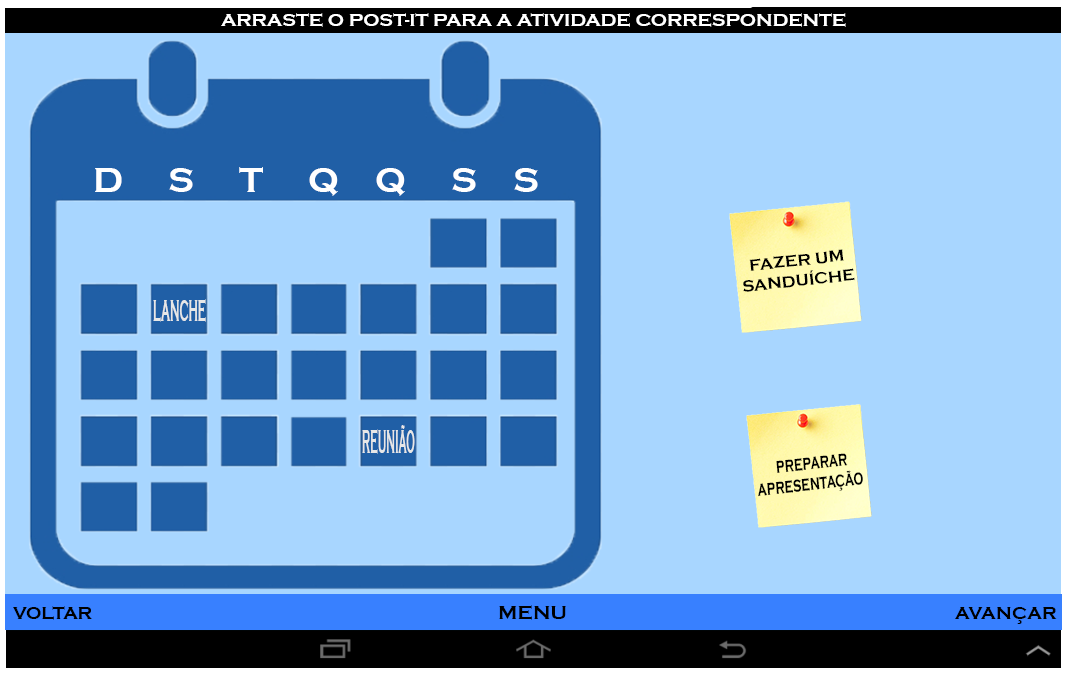
\includegraphics[width=1.0\textwidth]{emparelhamento_horarios.png}
    \caption{ Atividade Emparelhamento de Horário }
    \label{fig:emparelha_horario}
\end{figure}

Será apresentado ao usuário um calendário com algumas tarefas marcadas e alguns post-its com atividades para o usuário se preparar para as tarefas marcadas no calendário. Como pode ser visto na Figura \ref{fig:emparelha_horario}, é proposto ao usuário organizar os post-its de maneira a aproveitar ao máximo os horários vagos entre as tarefas, incentivando, assim, a prática de organização de horários.

\subsubsection{Emparelhamento de horário home-office}

 \begin{figure}[h!]
    \centering
    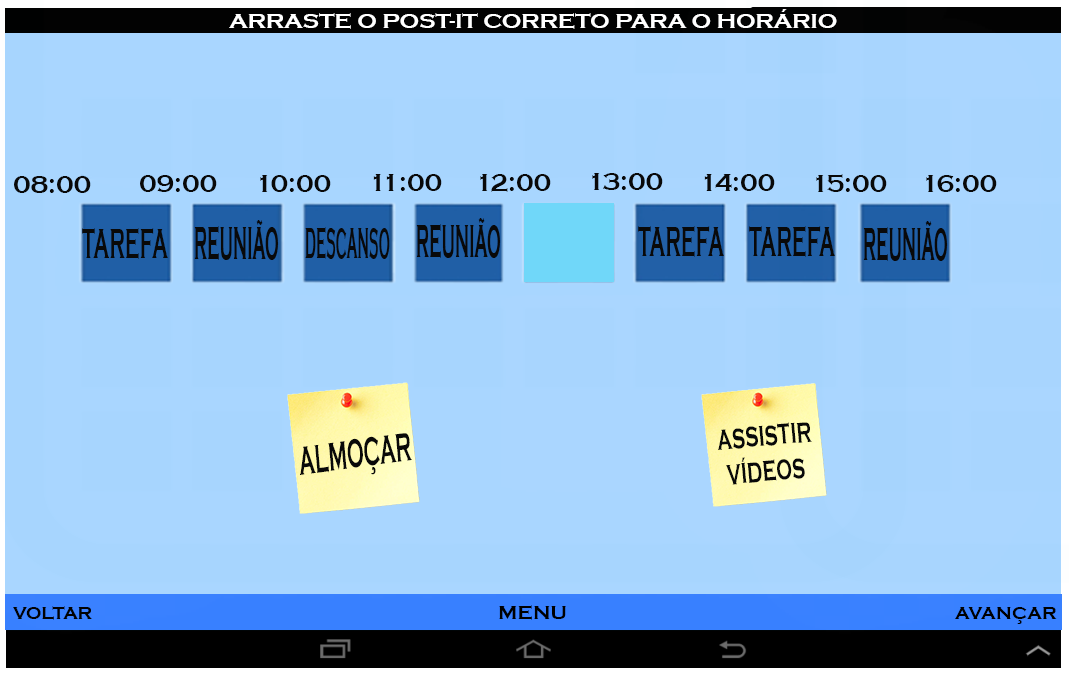
\includegraphics[width=1.0\textwidth]{emparelhamento_home_office.png}
    \caption{ Atividade Emparelhamento de Horário Home-Office }
    \label{fig:emparelha_home_office}
\end{figure}

A ideia aqui é transmitir ao usuário que é possível manter a boa prática de organizar bem seus horários mesmo em ambientes de trabalho à distância. Nesta atividade, mostrada na Figura \ref{fig:emparelha_home_office}, são acrescidos ao grupo de post-its para o usuário organizar novos post-its representando eventuais distrações e horários de descanso, para incentivar o usuário a distinguir um do outro, aprendendo assim a não praticar procrastinação.

\subsubsection{Dress-coding}

 \begin{figure}[h!]
    \centering
    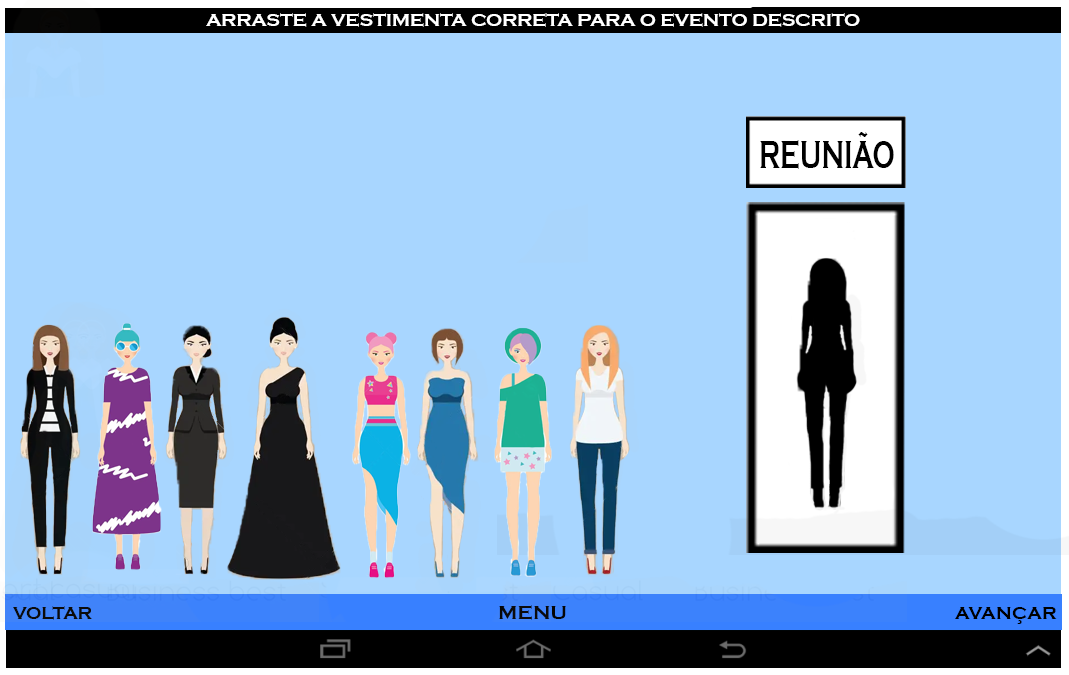
\includegraphics[width=1.0\textwidth]{dress_code.png}
    \caption{ Atividade de Dress Coding }
    \label{fig:dress_code}
\end{figure}

Esta atividade, referenciada na Figura \ref{fig:dress_code}, possui como objetivo dissertar ao usuário como uma flexibilização do dress-coding é tolerável conforme o contexto na qual ele se encontra. Serão apresentadas diferentes peças de roupa e uma caixa contendo o nome de um contexto (reunião, confraternização, "serviço normal", etc.). O usuário deve, então, arrastar para a caixa, quais peças de roupa ele vestiria dado determinado contexto. A fim de evitar que o colaborador decore que apenas uma peça de roupa é valida para aquela situação, múltiplas opções são aceitas como válidas para cada situação.

\subsubsection{Convivência}
 \begin{figure}[h!]
    \centering
    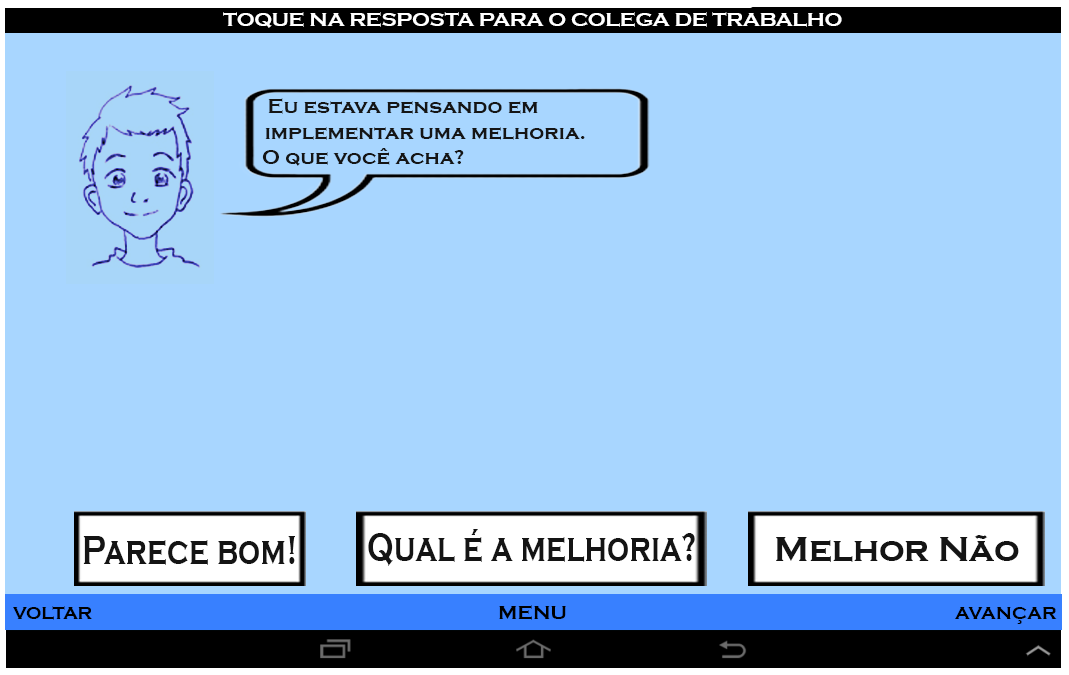
\includegraphics[width=1.0\textwidth]{convivencia1.png}
    \caption{ Atividade de Convivência }
    \label{fig:convivencia1}
\end{figure}
 \begin{figure}[h!]
    \centering
    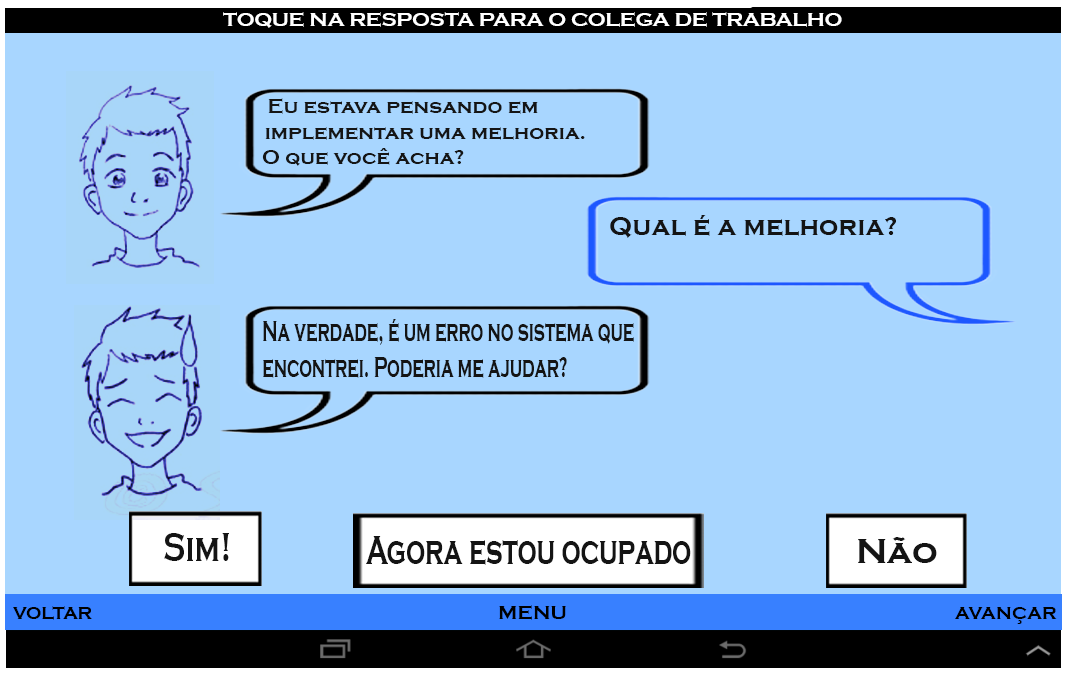
\includegraphics[width=1.0\textwidth]{convivencia2.png}
    \caption{ Atividade de Convivencia, o usuário escolheu a opção 'Qual é a melhoria?' }
    \label{fig:convivencia2}
\end{figure}
A proposta é apresentar ao usuário, nesta atividade, um jogo aventura-em-texto (text-adventure) para incentivar o mesmo a se socializar e comunicar propriamente com seus colegas de trabalho, externos e superiores.

São apresentados diferentes diálogos entre os diferentes membros do ambiente de trabalho na qual o usuário se encontra. Em seguida, é oferecido ao usuário algumas opções de resposta que levarão a diferentes novos diálogos conforme a resposta escolhida.

É interessante lembrar ao usuário, aqui, que situações reais são mais complexas e exigem mais prática para se escolher as melhores abordagens. O objetivo desta atividade não é necessariamente simular rigidamente uma situação real, mas incentivar o usuário a entender que, escolhendo uma abordagem aceitável e com boa comunicação (sendo educado), não há o que temer de simples conversas do dia-a-dia.

%o que vai entrar aqui que não entra na metodologia?
%R: metodologia descreve o que fizemos: usamos de base o documento da monografia do perceber 2 e adaptamos telas para um possivel software que cobrem tais atividades: (...)
% aqui descrevemos a fundo

\bibliographystyle{sbc}
\bibliography{sbc-template}

\end{document}
